\documentclass[fontsize=12pt,parskip=full,index=totoc,listof=totoc]{scrreprt}

\addtokomafont{disposition}{\rmfamily}
\addtokomafont{descriptionlabel}{\rmfamily}

\usepackage[ilines,headsepline]{scrpage2}
\pagestyle{scrheadings}
\clearscrheadfoot
\automark{section}
\ohead{\leftmark}
\cfoot{\pagemark}

\usepackage[utf8]{inputenc}
\usepackage[T1]{fontenc}
\usepackage[ngerman]{babel}

\usepackage{lmodern}
\usepackage{amsmath,amsfonts}
\usepackage{dsfont}
\usepackage{ellipsis}
\usepackage{microtype}
\usepackage{fixltx2e}
\usepackage{array}
\usepackage{longtable}
\usepackage{booktabs}
\usepackage{calc}
\usepackage{multirow}
\usepackage{xcolor}

\usepackage{scrhack}%entfernt warnmeldungen von listings
\usepackage{listings}
\lstset{basicstyle=\small\ttfamily}
\lstset{commentstyle=\slshape\color{blue!20!black}}
\lstset{showstringspaces=false}
\lstset{frame=leftline}
\lstset{mathescape=true}
\lstset{morecomment=[l][\color{blue!20!black}]{\#}}

\usepackage{makeidx}
\makeindex

\title{UMach Spezifikation}
\author{}

\usepackage[
    pdftitle={UMach VM Spezifikation},
    colorlinks=true,
    linkcolor=blue!50!black]
{hyperref} 

\usepackage[nonumberlist,toc]{glossaries}
\renewcommand*{\glspostdescription}{}% kein automatischer Punkt am Ende
\makeglossaries

% Glossary definitions
% Definition format: \newglossaryentry{label}{key=value...}
% Keys:
% name        - the name which will appear in text
% description - the description of the text, suround it with {}
% plural      - plural form
%
% Using a glossary term: 
% \gls{label}   for singular
% \glspl{label} for plural
% \Gls{label}   for first letter uppercase
% \Glspl{label} for first letter uppercase plural


\newglossaryentry{Adressierungsart}{
name={Adressierungsart},
description={Die Art, wie eine Instruktion die Umach Maschine dazu veranlasst,
einen Speicherbereich zu adressieren. Siehe auch Abschnitt
\ref{subsec:Adressierungsarten}.},
plural={Adressierungsarten}
}


\newglossaryentry{Byte}{
name=Byte,
description={Eine Reihe oder Gruppe von 8 Bit.},
plural={Bytes}
}

\newglossaryentry{Befehl}{
name=Befehl,
description={Die ersten 8 Bits in einer Instruktion. Operation code.},
plural={Befehle}
}

\newglossaryentry{Befehlsbreite}{
name=Befehlsbreite,
description={Die Länge eines Befehls in Bits. Ein UMach-Befehl ist 8 Bit lang.},
plural={Befehlsbreiten}
}

\newglossaryentry{Befehlsraum}{
name=Befehlsraum,
description={Die Anzahl der möglichen Befehle, abhängig von der
Befehlsbreite. Beträgt die Befehlsbreite $8$ Bit, so ist der Befehlsraum
$2^{8} = 256$.},
plural=Befehlsräume
}

\newglossaryentry{Instruktion}{
name=Instruktion,
description={Eine Anweisung an die UMach VM etwas zu tun. Eine Instruktion
besteht aus einem Befehl (Operation Code) und eventuellen Argumenten.},
plural={Instructionen}
}

\newglossaryentry{Instruktionsbreite}{
name=Instruktionsbreite,
description={Die Länge einer Instruktion in Bits. Eine UMach-Instruktion ist 32 Bit lang.},
plural={Instruktionsbreiten}
}

\newglossaryentry{Instruktionsformat}{
name={Instruktionsformat},
description={Beschreibt die Struktur einer Instruktion auf Byte-Ebene und zwar
es gibt an, ob ein Byte als eine Registerangabe oder als reine
numerische Angabe zu interpretieren ist. Siehe \ref{sec:Instruktionsformate}.},
plural={Instruktionsformate}
}

\newglossaryentry{Instruktionssatz}{
name=Instruktionssatz,
description={Die Menge aller Instruktionen, die von der UMach Maschine
ausgeführt werden können.},
plural=Instruktionssätze
}

\newglossaryentry{Register}{
name={Register},
description={Eine sich im Prozessor befindende Speichereinheit. Das Register
ist dem Programmierer sichbar und kann mit Werten geladen werden. Siehe
Abschnitt \ref{sec:Register}, Seite \pageref{sec:Register}.},
plural={Register}
}


% Ausgabe einer Befehlsdefinition in tabellarischer Form
% Nutzung: \opdef{<opname>}{<params>}{<opcode>}{<format>}
% opname: ADD, SUB etc
% params: Parameter
% opcode: hexa opcode
% format: Abschnitt Name eines Instruktionsformats
% Beispiel: \opdef{ADD}{X Y Z}{0x40}{RRR}
% Referenzieren mit \nameref{opcode:<opname>}
% Beispiel: \nameref{opcode:ADD}
\newcommand{\opdef}[4]{%
\subsection{\texttt{#1}}\index{#1@\texttt{#1}}%
\label{opcode:#1}%
\begin{center}%
  \begin{tabular}{llll}                       \toprule%
    Assemblername & Parameter & Maschinencode & Format \\\midrule%
    \texttt{#1}   & #2        & \texttt{#3}   & \nameref{#4}\\\bottomrule%
  \end{tabular}%
\end{center}%
}

% Die Menge aller Register bekommt ein eigenes Zeichen
\newcommand{\Reg}{\ensuremath{\mathcal{R}}}

\begin{document}
\maketitle
\tableofcontents

%--- Jedes Kapitel in eigener Datei und eigenem Verzeichnis 
%--- Jede Kapitel-Datei fängt mit \chapter an (markiert Kapitel)
%--- und kann nach belieben andere \section enthalten
%--- Empfehlung: jeder Abschnitt \section in eigener Datei

\chapter{Einführung}
UMach ist eine einfache virtuelle Maschine (VM), die einen definierten
Instruktionssatz und eine definierte Architektur hat. UMach orientiert
sich dabei an Prinzipien von RISC Architekturen: feste Instruktionslänge,
kleine Anzahl von einfachen Befehlen, Speicherzugriff durch Load- und
Store-Befehlen, u.s.w. Die UMach Maschine ist Register-basiert.
Der genaue Aufbau dieser Rechenmaschine ist im Abschnitt
\ref{sec:Aufbau} ab der Seite \pageref{sec:Aufbau} beschrieben.


Für den Anwender der virtuellen Maschine wird zuerst eine Assembler-Sprache zur
Verfügung gestellt. In dieser Sprache werden Programme geschrieben die
anschließend kompiliert werden. Die kompilierte Dateien (Maschinen-Code) wird
von der virtuellen Maschine ausgeführt.

\section{Anwendungsbeispiel}



\begin{lstlisting}
LOAD R1 90
LOAD R2 09
REV  R3 R1
\end{lstlisting}





\chapter{Organisation der UMach VM}

\section{Aufbau}
\index{UMach!Aufbau}
\label{sec:Aufbau}
Die virtuelle Maschine besteht aus einem Kern (der eigentlichen UMach Maschine)
und aus einem Bussystem. Das Bussystem wird im Abschnitt \ref{sec:Peripherie}
ab der Seite \pageref{sec:Peripherie} beschrieben.

Der Kern der Maschine besteht aus den folgenden Komponenten:

\begin{enumerate}
  \item Befehlsabruf Einheit (Instruction Fetch Unit)
  \item Decodierungseinheit
  \item Recheneinheit
  \item Register
\end{enumerate}

Die Decodierungseinheit ist dafür zuständig, eine abgerufene Instruktion zu
decodieren, bzw. in ihren Komponenten zu zerteilen.

Die Recheneinheit ist für die tatsächliche Ausführung der Instruktionen
zuständig. 

Die Register sind die Speichereinheiten, die sich in der Maschine befinden.



\subsection{Betriebsmodi}
\label{subsec:Betriebsmodi}
\index{Betriebsmodus}

Die Umach VM kann in zwei verschiedenen Betriebsmodi oder auch
Betriebsarten betrieben werden:

\begin{enumerate}
  \item Normalmodus
  \item Debugmodus
\end{enumerate}

\paragraph{Normalmodus} Die virtuelle Maschine führt alle Instruktionen
ohne Unterbrechung aus. Nach der Ausführung schaltet sich die Maschine aus.

\paragraph{Debugmodus} Die virtuelle Maschine führt immer nur eine
einzige Instruktion aus und bleibt dannach stehen. Um mit der folgenden
Instruktion fortzufahren wird immer ein externen Signal benötigt.
Dieser Modus soll dem Entwickler erlauben, ein Programm schrittweise zu
debuggen.

Der Modus kann vor dem Hochfahren der Maschine festgelegt, jedoch im
Betrieb nicht mehr geändert werden. Wird kein Modus angegeben, startet die
Maschine im Normalmodus.




\subsection{Register}
\index{Register}
\label{subsec:Register}

Der \gls{Register} sind die Speichereinheiten im Prozessor, die dem
Programmierer sichtbar sind.
Die meisten Anweisungen an die UMach Maschine bearbeiten auf einer Art diese
Register.


\subsection{Rechen- und logische Einheit}
\blindtext
\section{Speichermodell}
\index{Speichermodell}

\subsection{Adressierungsarten}
\label{subsec:Adressierungsarten}
\index{Adressierungsarten}

Als RISC-orientierte Maschine, greift die UMach lediglich in zwei Situationen
auf den Speicher zu: zum Schreiben von Registerinhalten in den Speicher
(Schreibzugriff) und zum Lesen von Speicherinhalten in einen Register
(Lesezugriff).  Die \gls{Adressierungsart} beschreibt dabei, wie der Zugriff
auf den Speicher erfolgen sollte, bzw. wie die angesprochene Speicheradresse
angegeben wird. Anders ausgedrückt, beantwortet die Adressierungsart die Frage
\glqq wie kann eine Instruktion der Maschine eine Adresse angeben?\grqq. 


Eine Instruktion kann die UMach Maschine auf zwei Arten dazu veranlassen,
den Speicher zu adressieren: 
\begin{enumerate}
  \item Direkte Adressierung
  \item Indirekte Adressierung
\end{enumerate}


\subsubsection{Direkte Adressierung}
\index{Adressierung!Direkte}

Die direkte Adressierung wird durch Angabe einer Speicheradresse spezifiziert.
Die Adresse wird in den letzten 2 Bytes einer Instruktion angeben. Diese
Instruktion hat das Format RNN (siehe auch \ref{subsec:RNN}). Eine Instruktion,
die die direkte Adressierung verwendet, hat also das folgende Format:
\begin{center}
  \begin{tabular}{|*{4}{c|}|c|} \hline
    erstes Byte    & zweites Byte  & drittes Byte  & viertes Byte & Algebraisch
\\\hline\hline
    Ladebefehl     & $R$ & \multicolumn{2}{c||}{Adresse $A$} &
    $R \gets mem(A)$ \\\hline
    Speicherbefehl & $R$ & \multicolumn{2}{c||}{Adresse $A$} &
    $R \to mem(A)$   \\\hline
  \end{tabular}
\end{center}
Die zweite Zeile weist die UMach Maschine an, dass sie den Inhalt der
angegebenen Speicheradresse $A$ (die letzten 2 Bytes) in das Register $R$ laden
soll. Die dritte Zeile gibt an, dass die Maschine den Inhalt des Registers $R$
an die angegebene Adresse $A$ schreiben (speichern) soll ($mem(x)$ steht für
Inhalt der Speicheradresse $x$).

Vorteil dieser Adressierungsart ist, dass sie keine zusätzliche Befehle zum
Lesen oder Schreiben in den Speicher benötigt. Nachteil ist, dass sie nur
Adressen angeben kann, die sich mit 16 Bit darstellen lassen. Adressen, die
größer als $2^{16} - 1$ sind können durch die zweite Adressierungsart angegeben
werden.


\subsubsection{Indirekte Adressierung}
\index{Adressierung!Indirekte}

Die indirekte Adressierung verwendet nicht, wie die direkte Adressierung,
ein Register und eine Speicheradresse, sondern zwei Register $B$ und $I$, die
von der Maschine verwendet werden um die endgültige Adresse zu berechnen:
Eine Instruktion, die diese Adressierung verwendet, hat also das Format RRR
(siehe auch \ref{subsec:RRR}).
\begin{center}
  \begin{tabular}{|*{4}{c|}|c|} \hline
    erstes Byte    & zweites Byte  & drittes Byte  & viertes Byte & Algebraisch
\\\hline\hline
    Ladebefehl     & $R$  & $B$  & $I$  & $R \gets mem(B + I)$ \\\hline
    Speicherbefehl & $R$  & $B$  & $I$  & $R \to   mem(B + I)$ \\\hline
  \end{tabular}
\end{center}
Die fünfte Spalte gibt jeweils den äquivalenten algebraischen Ausdruck wieder.
$mem(x)$ steht dabei für den Inhalt der Adresse $x$.


Die zweite Zeile (Ladebefehl) bedeutet, dass die UMach Maschine die Inhalte der
Register $B$ und $I$ aufaddieren soll, diese Summe als absolute Adresse im
Speicher zu verwenden und den Inhalt an dieser Adresse in den Register $R$ zu
kopieren.

Die dritte Zeile (Speicherbefehl) bedeutet: die Maschine soll den Inhalt des
Registers $R$ an die Adresse $B + I$ schreiben.

Üblicherweise enthält $B$ eine Startadresse und $I$ einen Versatz oder Index zur
Adresse in $B$.

Vorteil der indirekten Adressierung ist, dass sie $2^{33} - 1$ mögliche
Adressen ansprechen kann.
Nachteil ist, dass zwei oder mehrere Instruktionen gebraucht werden, um diese
Adressierung zu verwenden, denn die Register $B$ und $I$ erst entsprechend geladen
werden müssen.

Die Register $R$, $B$ und $I$ stehen für beliebige Register.

\input{organisation/Datentypen}


\chapter{Instruktionssatz}
\label{chap:Instruktionssatz}
\index{Instruktionssatz}

In diesem Kapitel werden alle Instruktionen\index{Instruktionen} der UMach VM 
vorgestellt.

\section{Allgemeines}

\section{Instruktionsformate}
\index{Instruktionsformat}

\paragraph{Instruktionsbreite}
\index{Instruktionsbreite}
Jede UMach-Instruktion hat eine feste Bitlänge von 32 Bit (4 mal 8 Bit).
Das gilt unabhängig davon, was die Instruktion tut. Instruktionen, die für ihren
Informationsgehalt weniger als 32 Bit brauchen, wie z.B. \texttt{NOP},
werden mit Nullbits gefüllt. Alle Daten und Informationen, die mit einer
Instruktion übergeben werden, müssen in diesen 32 Bit untergebracht werden.

\paragraph{Byte Order}
\index{Byte Order}
Die Byte Order (Endianness) der gelesenen \glspl{Byte} ist
big-endian, die Byte-Reihenfolge, die für den Mensch selbstverständlich wäre
(von links nach rechts lesen):
die zuerst gelesenen 8 Bits sind die 8 höchstwertigen (Wertigkeiten $2^{31}$ bis
$2^{24}$) und die zuletzt gelesenen Bits sind die niedrigstwertigen
(Wertigkeiten $2^{7}$ bis $2^{0}$).
Bits werden in Stücken von $n$ Bits gelesen, wobei $n = k \cdot 8$ und
$k \in \mathbb{N} \setminus\{0\}$ (Byte für Byte).


\paragraph{Allgemeines Format}
Jede \gls{Instruktion} besteht aus zwei Teilen: der erste Teil ist
8 Bit lang und entspricht dem tatsächlichen \gls{Befehl}, bzw. der Operation,
die von der UMach virtuellen Maschine ausgeführt werden soll.
Dieser 8-Bit-Befehl belegt also die 8 höchstwertigen Bits einer Instruktion.
Die übrigen 24 Bit werden für Operanden oder Daten benutzt. Beispiel einer
Instruktionszerlegung:

\begin{center}
  \begin{tabular}{|l|*{4}{c|}}
    \hline
    Instruktion &
    \texttt{00000001} & \texttt{00000010} & \texttt{00000011} & \texttt{00000100}
    \\\hline
    Hexa  &
    \texttt{01}   & \texttt{02}   & \texttt{03}   & \texttt{04}
    \\\hline
    Byte Order &
    erstes Byte   & zweites Byte  & drittes Byte  & viertes Byte
    \\\hline
    Interpretation &
    Befehl    &  \multicolumn{3}{c|}{Operanden, Daten oder Füllbits}
    \\\hline
  \end{tabular}
\end{center}

Die Instruktionsformate unterscheiden sich lediglich darin, dass sie die 24 Bits
nach dem 8-Bitigen \gls{Befehl} unterschiedlich verwenden.


\section{Verteilung des Befehlsraums}
\index{Befehlsraum}
Zur besseren Übersicht der verschiedenen UMach-\glspl{Instruktion}, unterteilen
wir den \gls{Instruktionssatz} der UMach virtuellen Maschine in den folgenden
Kategorien:
\index{Instruktionen!Kategorien}

\index{Befehlsraum!Verteilung}
\begin{enumerate}
  \item Kontrollinstruktionen,  die die Maschine in ihrer gesamten
    Funktionalität betreffen, wie z.B. den Betriebsmodus umschalten.
  \item Lade- und Speicherbefehle, die Register mit Werten aus dem Speicher, 
    anderen Registern oder direkten numerischen Angaben laden und die
    Registerinhalte in den Speicher schreiben.
  \item Arithmetische Instruktionen, die einfache arithmetische Operationen
    zwischen Registern veranlassen.
  \item Logische Instruktionen, die logische Verknüpfungen zwischen
    Registerinhalten oder Operationen auf Bit-Ebene in Registern anweisen.
  \item Vergleichsinstruktionen, die einen Vergleich zwischen
    Registerinhalten angeben.
  \item Sprunginstruktionen, die bedingt oder unbedingt sein können.
    Sie weisen die UMach Maschine an, die Programmausführung an einer anderen
    Stelle fortzufahren.
  \item Unterprogramm-Steuerung, bzw. Instruktionen, die die Ausführung von
    Unterprogrammen (Subroutinen) steuern.
  \item Systeminstruktionen, die die Unterstützung eines
    Betriebssystem ermöglichen.
\end{enumerate}

Die oben angegebenen Instruktionskategorien unterteilen den \gls{Befehlsraum} in
8 Bereiche. Es gibt $256$ mögliche Befehle, gemäß $2^{8} = 256$.
Die Verteilung der Kategorien auf die verschiedenen Maschinencode-Intervallen
wird in der Tabelle \ref{tab:Befehlraumverteilung} auf Seite
\pageref{tab:Befehlraumverteilung} angegeben.

\input{instruktionen/Verteilung-Tabelle}
\input{instruktionen/Instruktionen-Tabelle}

Die Tabelle \ref{tab:Befehlentabelle} auf der Seite 
\pageref{tab:Befehlentabelle} enthält eine Übersicht aller Befehle und
deren Maschinencodes.
Diese Tabelle wird folgenderweise gelesen:
in der am weitesten linken Spalte wird die erste hexadezimale Ziffer eines
Befehls angegeben (ein Befehl ist zweistellig im Hexadezimalsystem).
Jede solche Ziffer hat rechts Zwei Zeilen, die von links nach rechts gelesen
werden: eine Zeile für die Ziffern von 0 bis 8, die anderen für die übrigen
Ziffern 9 bis F (im Hexadezimalsystem). Die Assemblernamen (Mnemonics) der
einzelnen Befehle sind an der entsprechenden Stelle angegeben.

\paragraph{Definitionsstruktur}
Im den folgenden Abschnitten werden die einzelnen Instruktionen beschrieben. Zu
jeder Instruktion wird der \gls{Assemblername}, die Parameter, der Maschinencode
(\gls{Maschinenname}) und das Instruktionsformat, das die Typen der Parameter
definiert, formal angegeben. Zudem werden Anwendungsbeispiele angegeben. Die
Instruktionsformate können im Abschnitt \ref{sec:Instruktionsformate} ab der
Seite \pageref{sec:Instruktionsformate} nachgeschlagen werden.

\paragraph{Zur Notation}
Mit \Reg\index{\Reg} wird die Menge aller Register
gekennzeichnet\footnote{Nicht verwechseln mit den Symbolen $\mathds{R}$ und
$\mathbb{R}$, die die Menge aller reellen Zahlen bedeuten.}.
Die Notation $X \in \Reg$ bedeutet, dass $X$ ein Element aus dieser Menge ist,
mit anderen Worten, dass $X$ ein Register ist. Analog bedeutet die
Schreibweise $X,Y \in \Reg$, dass $X$ und $Y$ beide Register sind.

Gilt $X, Y\in \Reg$ und ist $\sim$ eine durch einen Befehl definierte Relation
zwischen $X$ und $Y$, so bezieht sich die Schreibweise $X \sim Y$ nicht auf die
Maschinennamen von $X$ und $Y$, sondern auf deren Inhalte. Zum Beispiel, haben
die Register $R1$ und $R2$ die Maschinencodes \texttt{0x01} und \texttt{0x02}
und sind sie mit den Werten $4$ bzw. $5$ belegt, so bedeutet $R1 + R2$ das
gleiche wie $4 + 5 = 9$ und nicht \texttt{0x01 + 0x02 = 0x03}.

Andere verwendeten Schreibweisen:
\begin{center}
\begin{tabular}{l|l}\toprule
 $\mathds{N}$ & Menge aller natürlichen Zahlen: $0,1,2,\ldots$         \\
 $\mathds{Z}$ & Menge aller ganzen Zahlen: $\ldots,-2,-1,0,1,2,\ldots$ \\
 $N \in \mathds{N}$
              & $N$ ist Element von $\mathds{N}$, oder liegt im Bereich von
              $\mathds{N}$                                             \\
 $X \gets Y$  & $X$ wird auf $Y$ gesetzt                               \\
 $mem(X)$     & Speicherinhalt an der Adresse $X$ (1 Byte)             \\
 $mem_{n}(X)$ & Speicherinhalt an der Adresse $X$ ($n$ Bytes)          \\
\bottomrule
\end{tabular}
\end{center} 

\subsection{Notationen}
\index{Notation}


Mit \Reg\index{\Reg} wird die Menge aller Register
gekennzeichnet\footnote{Nicht verwechseln mit den Symbolen $\mathds{R}$ und
$\mathbb{R}$, die die Menge aller reellen Zahlen bedeuten.}.
Die Notation $X \in \Reg$ bedeutet, dass $X$ ein Element aus dieser Menge ist,
mit anderen Worten, dass $X$ ein Register ist. Analog bedeutet die
Schreibweise $X,Y \in \Reg$, dass $X$ und $Y$ beide Register sind.


Wenn $X$ ein Register bezeichnet, dann bezeichnet $\$X$ den Inhalt des
Registers $X$. Diese Notation wird verwendet, um in Aussagen wie 
\glqq $\$X + \$Y$\grqq\ klar zu machen, dass es sich um die Registerinhalte von
$X$ und $Y$ handelt, nicht um die Register selbst.

Die Tabelle \ref{tab:Notationen} auf der Seite \pageref{tab:Notationen}
wiedergibt alle Notationen, die in diesem Kapitel verwendet werden.

\begin{longtable}{ll}
 \caption{Verwendete Notationen}
 \label{tab:Notationen}
 \\\toprule
 Notation & Bedeutung \\\midrule
 \endfirsthead
 \\\toprule
 Notation & Bedeutung \\\midrule
 \endhead
 $\mathds{N}$ & Menge aller natürlichen Zahlen: $0,1,2,\ldots$         \\
 $\mathds{N}_{\setminus 0}$ 
              & $\mathds{N}$ ohne die Null: $1,2,\ldots$               \\
 $\mathds{Z}$ & Menge aller ganzen Zahlen: $\ldots,-2,-1,0,1,2,\ldots$ \\
 $\mathds{Z}_{\setminus 0}$ 
              & $\mathds{Z}$ ohne die Null: $\ldots,-2,-1,1,2,\ldots$  \\
 $N \in \mathds{N}$
              & $N$ ist Element von $\mathds{N}$, oder liegt im Bereich von
              $\mathds{N}$                                             \\
 $\Reg$       & Menge aller Register                                   \\
 $X \in \Reg$ & $X$ ist ein Register                                   \\
 $\$X$        & Inhalt des Registers $X$                               \\
 $a \gets b$  & $a$ wird auf $b$ gesetzt                               \\
 $X \gets \$Y$& $X$ wird auf den Inhalt des Registers $Y$ gesetzt      \\
 $mem(X)$     & Speicherinhalt an der Adresse $X$ (1 Byte)             \\
 $mem_{n}(X)$ & $n$-Bytes-Block im Speicher ab Adresse $X$             \\
 \texttt{mem[n]}
              & äquivalent zu $mem(n)$                                 \\
 $lsb_{n}(X)$ \index{las@$lsb$}
              & \glqq least significant $n$ bits\grqq\ von $X$        \\
 \bottomrule
\end{longtable}



\section{Kontrollinstruktionen}

\opdef{NOP}{keine}{0x00}{000}
Diese Instruktion (\glqq No Operation\grqq) bewirkt nichts.
Der Sinn dieser Instruktion ist, den Maschinencode mit Nullen füllen zu können,
ohne dabei die gesamte Ausführung zu beeinflussen, außer, Zeitlupen zu schaffen. 


\opdef{RST}{keine}{0x01}{000}
Setzt alle Register außer dem Befehlszähler auf Null.


\opdef{CRM}{$N \in \mathds{N}$}{0x02}{NNN}
\glqq Change Run Mode\grqq.
Setzt das \gls{Betriebsmodus}.\index{Betriebsmodus}
Dabei ist das Parameter einer der folgenden konstanten Werten:
\begin{center}
  \begin{tabular}[l]{ll}
    0 & Normalmodus \\
    1 & Einzelschrittmodus \\
  \end{tabular}
\end{center}
Siehe Abschnitt \ref{subsec:Betriebsmodi} auf Seite
\pageref{subsec:Betriebsmodi}.



\opdef{CSM}{$N \in \mathds{N}$}{0x03}{NNN}
Change System Mode.



\opdef{DIE}{keine}{0x04}{000}
Die Maschine ausschalten.



\opdef{RSR}{keine}{0x05}{000}
\glqq Resurrect\grqq.
Die Maschine neustarten.



\opdef{AUTSM}{keine}{0x06}{000}
\glqq Become autistic\grqq.
Bewirkt, dass alle Lese- und Schreibbefehle, die sich nicht ausschließlich auf
Register beziehen, wirkungslos sind. Praktisch wird die Kommunikation mit dem
Bussystem ausgeschaltet.


\opdef{SOCL}{keine}{0x07}{000}
\glqq Become social\grqq. Schaltet die Kommunikation mit dem Bussystem ein.


\opdef{HATE}{keine}{0x08}{000}
\glqq Hate\grqq. Schaltet alle Schutzmechanismen ein.


\opdef{TRST}{keine}{0x09}{000}
\glqq Trust\grqq. Schaltet alle Schutzmechanismen aus.


\opdef{ZMB}{keine}{0x0A}{000}
\glqq Become a zombie\grqq.
Schaltet alle Registeränderungen aus. Nach der Ausführung dieses Befehls, alle
Operationen, die einen Register modifizieren sollen, sind wirkungslos.
Die Maschine ändert ihren Zustand nicht mehr, außer, dass sie weitere Befehle
liest.


\opdef{ALIV}{keine}{0x0B}{000}
\glqq Become alive\grqq.
Nach der Ausführung dieses Befehls, alle Register können wie normal modifiziert
werden.



\section{Lade- und Speicherbefehle}
\label{sec:Lade-Speicher-Instruktionen}

\opdef{SET}{$X\in\Reg$, $N\in\mathds{Z}$}{0x10}{RNN}
Setzt den Inhalt des Registers $X$ auf den ganzzahligen Wert $N$.
Da $N$ mit 16 Bit und im Zweierkomplement dargestellt wird, kann $N$ Werte von
$-2^{15}$ bis $2^{15} - 1$ aufnehmen, bzw. von $-32768$ bis $+32767$.
Werte außerhalb dieses Intervalls werden auf Assembler-Ebene entsprechend
gekürzt (es wird modulo berechnet, bzw. nur die ersten 16 Bits aufgenommen).

Beispiele:
\begin{lstlisting}
label:
  SET R1  8    # $R1 \gets 8$
  SET R2 -3    # $R2 \gets -3$
  SET R3 65536 # $R3 \gets 0$, da $65536 = 2^{16} \equiv 0 \bmod 2^{16}$
  SET R4 70000 # $R3 \gets 4464 = 70000 \bmod 2^{16}$
  SET R7 label # Adresse 'label' ins R7
\end{lstlisting}


\opdef{CP}{$X, Y \in \Reg$}{0x11}{RR0}
\glqq Copy\grqq.
Kopiert den Inhalt des Registers $Y$ in das Register $X$. Register $Y$ wird
dabei nicht geändert. Entspricht
\[
    X \gets \$Y
\]

Beispiel:
\begin{lstlisting}
 SET  R1 5  # $R1 \gets 5$
 CP   R2 R1 # $R2 \gets 5$
\end{lstlisting}



\opdef{LB}{$X, Y \in \Reg$}{0x12}{RR0}
Lade ein Byte aus dem Speicher mit Adresse $\$Y$ in das niedrigstwertige
Byte des Registers $X$. Die anderen Bytes von $X$ werden von diesem Befehl nicht
geändert. Insbesondere, werden sie nicht auf Null gesetzt.

Äquivalenter C Code:
\begin{lstlisting}
  x = (x & 0xFFFFFF00) | (mem(y) & 0x00FF);
\end{lstlisting}

Entspricht 
\[
  lsb_{8}(X) \gets mem(\$Y)
\]
(siehe Tabelle \ref{tab:Notationen} auf Seite \pageref{tab:Notationen} für die
Notationen).

\paragraph{Fehler}
Falls der Inhalt des Registers $Y$ eine ungültige Speicheradresse ist, wird der
Interrupt mit Nummer 16 (ungültige Speicheradresse) generiert und das Bit mit
Nummer 8 im Register \texttt{ERR} gesetzt.


\paragraph{Beispiel}
Angenommen, der Speicher an den Adressen $100$ und $101$ hat den Wert $5$, bzw.
$6$. Dann können diese zwei nacheinander folgenden Bytes auf die
folgende Weise in $R2$ gelesen werden. $R1$ wird dabei als Zeiger im Speicher
verwendet.
\begin{lstlisting}
  SET  R1     100   # Speicheradresse R1 = 100
  SET  R2       0
  LB   R2  R1       # R2 = 5 ($mem(100)$)
  SHLI R2  R2   8   # shift left 8 Bit, R2 = 1280
  INC  R1           # R1++, R1 = 101
  LB   R2  R1       # R2 = 1286 (R2 + $mem(101)$)
\end{lstlisting}




\opdef{LW}{$X, Y \in \Reg$}{0x13}{RR0}
\glqq Load Word\grqq.
Lade ein Wort (4 Byte) aus dem Speicher mit Adresse $\$Y$ in das Register $X$.
Alle Bytes von $X$ werden dabei überschrieben. Die Bytes aus dem Speicher werden
nacheinander gelesen. Es werden also die Bytes mit Adressen $\$Y + 0$, $\$Y +
1$, $\$Y + 2$ und $\$Y + 3$ zu einem 4-Byte Wort zusammengesetzt und so in $X$
ablegt.

Entspricht 
\[
  X \gets mem_{4}(\$Y)
\]

\paragraph{Fehler}
Wie bei der Instruktion \opref{LB}.


\paragraph{Bemerkung}
Die UMach Maschine verwendet stets die \glqq big-endian\grqq\ Byte-Reihenfolge.


\paragraph{Beispiel}
Angenommen, die Adressen von 100 bis 103 sind mit den Werten 0, 1, 2 und 3
belegt und bilden somit den Wert $66051$.
\begin{lstlisting}
  SET R1   100
  LW  R2 R1     # $R2 \gets mem_{4}(R1) = 66051$
\end{lstlisting}




\opdef{SB}{$X, Y \in \Reg$}{0x14}{RR0}
\glqq Store Byte\grqq.
Speichert den Inhalt des niedrigstwertigen Byte von $X$ an der Speicheradresse
$\$Y$. $X$ und $Y$ sind dabei Register.

Entspricht
\[
    \$X \to mem_{1} (\$Y)
\]
$mem_{1}(x)$ bedeutet dabei 1 Byte an der Adresse $x$.

\paragraph{Fehler}
Falls der Inhalt des Registers $Y$ eine ungültige Speicheradresse ist, wird der
Interrupt mit Nummer 16 (ungültige Speicheradresse) generiert und das Bit mit
Nummer 8 im Register \texttt{ERR} gesetzt. Falls die Speicheradresse $\$Y$
schreibgeschützt ist, wird der Interrupt mit Nummer 17 (Zugriffsverletzung)
erzeugt und das Bit mit Nummer 9 im Register \texttt{ERR} gesetzt..

\paragraph{Beispiel}
\begin{lstlisting}
  SET R1 128     # R1 = Speicheradresse 128
  SET R2 513     # R2 = 0x0201
  SB  R2 R1      # Speicher mit Adresse 128 wird auf 1 gesetzt
\end{lstlisting}




\opdef{SW}{$X, Y\in \Reg$}{0x15}{RR0}
\glqq Store Word\grqq.
Speichert den Inhalt aller Bytes in $X$ an die Speicheradressen $\$Y$ bis 
$\$Y + 3$.
\[
    \$X \to mem_{4}(\$Y)
\]

\paragraph{Fehler}
Wie bei \opref{SB}, nur auf den ganzen Speicherbereich $\$Y$ bis $\$Y + 3$
bezogen.


\paragraph{Beispiel}
Es wird das Register $R2$ mit dem Wert \texttt{0x01020304} geladen und an die
Adresse $128$ gespeichert. Dabei werden die Byte-Werten in 
\glqq big-endian\grqq\ Reihenfolge gespeichert: das höchstwertige Byte aus $R2$
(\texttt{0x01}) wird an der Adresse $128$ gespeichert, das niedrigstwertige
Byte (\texttt{0x04}) an die Adresse $131$.

\begin{lstlisting}
  SET R1 128         # R1 = Speicheradresse 128
  SET R2 0x01020304  # Wert zum Speichern
  SH  R2 R1          # mem[128] = 0x01
                     # mem[129] = 0x02
                     # mem[130] = 0x03
                     # mem[131] = 0x04
\end{lstlisting}




\opdef{PUSH}{$X \in \Reg$}{0x18}{R00}
\glqq Push Word\grqq.
Erniedrigt das Register \texttt{SP} um 4 und kopiert das ganze Register $X$ auf
den Stack, wobei der \glqq Stack\grqq\ ist der Speicherbereich mit
Anfangsadresse in \texttt{SP}.
Die Byte-Reihenfolge der Lese- und Schreiboperationen ist \glqq Big-Endian\grqq\
und wird in der nachfolgenden Tabelle dargestellt:
\begin{center}
\begin{tabular}{l|cccc}
  \toprule
  $X$  Wertigkeiten &
  $2^{31} \leftrightarrow 2^{24}$ &
  $2^{23} \leftrightarrow 2^{16}$ &
  $2^{15} \leftrightarrow 2^{8}$  &
  $2^{7}  \leftrightarrow 2^{0}$ 
  \\
  &
  $\downarrow$ & $\downarrow$ & $\downarrow$ & $\downarrow$ 
  \\
  \text{Stack-Bereich} &
  \texttt{mem[SP + 0]} &
  \texttt{mem[SP + 1]} &
  \texttt{mem[SP + 2]} &
  \texttt{mem[SP + 3]}
  \\\bottomrule
\end{tabular}
\end{center}


Entspricht
\begin{align*}
   SP & \gets \$SP - 4    \\
 \$X  & \to mem_{4}(SP)
\end{align*}


\paragraph{Fehler}
Falls die Verringerung $\$SP - 4$ eine Speicheradresse außerhalb des
Stackbereichs ergibt, d.h. wenn $(\$SP -4) \leq \$HE$, wird der Interrupt mit
Nummer 26 (Stack Überlauf) \index{Stack!Überlauf} generiert und das Bit mit
Nummer 11 im Register \texttt{ERR} gesetzt. Dabei beinhaltet das Register $HE$
die Adresse des letzten Bytes im Heap-Segment. Siehe auch den Abschnitt
\ref{subsec:Stack} auf der Seite \pageref{subsec:Stack}, sowie den Abschnitt
\ref{subsec:Speicherfehler} auf der Seite \pageref{subsec:Speicherfehler}.


\paragraph{Beispiel}
Der folgende Code speichert das 4-Byte Wort \texttt{0x01020304} auf den Stack.
Die Stack-Struktur wird in Kommentaren gezeigt.
\begin{lstlisting}
  SET  R1 0x01020304 # Wert zum pushen
  PUSH R1            # mem[SP + 0] = 0x01
                     # mem[SP + 1] = 0x02
                     # mem[SP + 2] = 0x03
                     # mem[SP + 3] = 0x04
                     # $\$SP \gets \$SP - 4$
\end{lstlisting}




\opdef{POP}{$X \in \Reg$}{0x19}{R00}
\glqq Pop Word\grqq.
Speichert 4 Bytes ab der Adresse $\$SP$ in das Register $X$ und erhöht $\$SP$ um
4. Die Byte-Reihenfolge der Lese- und Schreiboperationen ist \glqq
Big-Endian\grqq\ und wird in der nachfolgenden Tabelle dargestellt.

\begin{center}
\begin{tabular}{l|cccc}
  \toprule
  $X$  Wertigkeiten &
  $2^{31} \leftrightarrow 2^{24}$ &
  $2^{23} \leftrightarrow 2^{16}$ &
  $2^{15} \leftrightarrow 2^{8}$  &
  $2^{7}  \leftrightarrow 2^{0}$ 
  \\
  &
  $\uparrow$ & $\uparrow$ & $\uparrow$ & $\uparrow$ 
  \\
  \text{Stack-Bereich} &
  \texttt{mem[\$SP + 0]} &
  \texttt{mem[\$SP + 1]} &
  \texttt{mem[\$SP + 2]} &
  \texttt{mem[\$SP + 3]}
  \\\bottomrule
\end{tabular}
\end{center}

Entspricht
\begin{align*}
  X  & \gets mem_{4}(\$SP) \\
  SP & \gets \$SP + 4
\end{align*}


\paragraph{Fehler}
Falls das Register \texttt{SP} zu einer Adresse außerhalb des Stackbereichs
zeigt, wird der Interrupt mit Nummer 16 (ungültige Speicheradresse)
generiert und das Bit mit Nummer 8 im Register \texttt{ERR} gesetzt.


\paragraph{Beispiel}
Angenommen, die ersten 4 Bytes auf dem Stack (d.h. ab der Adresse, die im
Register \texttt{SP} angegeben ist) sind \texttt{0xAA 0xBB 0xCC 0xDD}.
\begin{lstlisting}
  POPH R1      # R1 = 0xAABBCCDD
               # $\$SP \gets \$SP + 4$
\end{lstlisting}

\section{Arithmetische Instruktionen} 

\opdef{ADD}{$X,Y,Z \in \Reg$}{0x50}{RRR}
Vorzeichen behaftete Addition der Registerinhalte $Y$ und $Z$.
Das Ergebnis der Addition wird in das Register $X$ gespeichert.
Entspricht dem algebraischen Ausdruck
\[
    X \gets Y + Z
\]
Beispiel:
\begin{lstlisting}
  SET   R1 1     # $R1 \gets 1$
  SET   R2 2     # $R2 \gets 2$
  ADD   R3 R1 R2 # $R3 \gets R1 + R2 = 1 + 2 = 3$
  #     X  Y  Z
  SET   R2 -2    # $R2 \gets -2$
  ADD   R3 R3 R2 # $R3 \gets R3 + R2 = 3 +(-2) = 1$
  ADD   R3 R4  5 # Fehler! 5 kein Register
\end{lstlisting}
Vorzeichenlose Addition wird durch den Befehl \texttt{ADDU} ausgeführt.


\opdef{ADDU}{$X,Y,Z \in \Reg$}{0x51}{RRR}
\glqq Add Unsigned\grqq.
Vorzeichenlose Addition der Register $Y$ und $Z$. Das Ergebnis wird in das
Register $X$ gespeichert. Enthält $Y$ oder $Z$ ein Vorzeichen (höchstwertiges
Bit auf 1 gesetzt), so wird es nicht als solches interpretiert, sondern als
Wertigkeit, die zum Betrag des Wertes hinzuaddiert wird ($+2^{31}$).

\begin{lstlisting}
  SET   R1 1     # $R1 \gets 1$
  SET   R2 -2    # $R2 \gets -2$
  ADDU  R3 R1 R2 # $R3 \gets (1 + 2 + 2^{31}) = 2147483651$
\end{lstlisting}



\opdef{ADDI}{$X,Y\in\Reg$, $N\in\mathds{Z}$}{0x52}{RRN}
\glqq Add Immediate\grqq.
Hinzuaddieren eines festen vorzeichenbehafteten ganzzahligen Wert $N$ zum Inhalt
des Registers $Y$ und speichern des Ergebnisses in das Register $X$.
Entspricht dem algebraischen Ausdruck
\[
  X \gets Y + N
\]
$N$ wird als vorzeichenbehaftete 8-Bit Zahl in Zweierkomplement-Darstellung
interpretiert und kann entsprechend Werte von $-128$ bis $127$ aufnehmen.

Beispiel:
\begin{lstlisting}
  SET   R1 1     # $R1 \gets 1$
  ADDI  R2 R1 2  # $R2 \gets R1 + 2 = 1 + 2 = 3$
  #     X  Y  N
  ADDI  R2 R2 -3 # $R2 \gets R2 + (-3) = 3 +(-2) = 1$
  ADDI  R2 R3 R4 # Fehler! R4 kein $n \in \mathds{Z}$
\end{lstlisting}



\opdef{ADDIU}{$X,Y \in \Reg$, $N\in\mathds{N}$}{0x53}{RRN}
\glqq Add Unsigned Immediate\grqq.
Vorzeichenlose Addition des ganzzahligen Wertes $N$ zum Inhalt des Registers $Y$
und speichern des Ergebnisses in das Register $X$.
Der Inhalt des Registers $Y$, die Zahl $N$ und das Ergebnis $Y + N$ werden als
vorzeichenlose Werte interpretiert.
Die Feste natürliche Zahl $N$ kann Werte aus dem Bereich $[0, 255]$ aufnehmen.
Wird eine größere Zahl angegeben, so wird sie modulo $256$ berechnet.



\opdef{SUB}{$X, Y, Z \in \Reg$}{0x58}{RRR}
Subtrahiert die Registerinhalte von $Y$ und $Z$ und speichert das Ergebnis in
das Register $X$. Entspricht dem Ausdruck
\[
    X \gets (Y - Z)
\]
Wobei $X$, $Y$ und $Z$ Register sind.



\opdef{SUBU}{$X, Y, Z \in \Reg$}{0x59}{RRR}
\glqq Subtract Unsigned\grqq.
Analog zur Instruktion \opref{SUB} mit dem Unterschied, dass alle Werte und
Operationen vorzeichenlos sind.


\opdef{SUBI}{$X, Y \in \Reg$, $N\in\mathds{Z}$}{0x5A}{RRN}
\glqq Subtract Immediate\grqq.
Funktioniert wie \opref{SUB} aber $N$ ist eine direkt angegebene Zahl
(kein Register).

\paragraph{Beispiel}
Folgendes Beispiel demonstriert die Verwendung von \opref{SUBI} und zeigt
zugleich einen Fehler.
\begin{lstlisting}
  SET  R1 50     # $R1 \gets 50$
  SUBI R2 R1 30  # $R2 \gets (R1 - 30) = 20$
  SUBI R2 R1 R1  # Fehler! da $R1 \not\in \mathds{Z}$
\end{lstlisting}


\opdef{SUBIU}{$X, Y \in \Reg$, $N\in\mathds{N}$}{0x5B}{RRN}
\glqq Subtract Immediate Unsigned\grqq.
Funktioniert wie die Instruktion \opref{SUBI} mit dem Unterschied, dass
\opref{SUBIU} ausschliesslich mit vorzeichenlosen Werten arbeitet. 



\opdef{MUL}{$X, Y \in \Reg$}{0x60}{RR0}
\glqq Multiply\grqq. 
Multipliziert die Inhalte der Register $X$ und $Y$ und speichert das Ergebnis in
die Spezialregister \texttt{HI} und \texttt{LO}. Diese zwei Spezialregister
werden als eine 64-Bit Einheit betrachtet, wobei jedes eine Hälfte des
64-Bit Ergebnisses enthält.
Dabei werden die höchstwertigen 32 Bit des Ergebnisses in das Register
\texttt{HI}\index{HI@\texttt{HI}}
und die 32 niedrigstwertigen Bits des Ergebnisses in das Register
\texttt{LO}\index{LO@\texttt{LO}} gespeichert.
Siehe auch die Tabelle \ref{tab:Spezialregister} auf der Seite
\pageref{tab:Spezialregister}.

Falls das Ergebnis der Multiplikation gänzlich in den 32 Bit des Registers
\texttt{LO} passt, wird das Register \texttt{HI} trotzdem auf Null gesetzt.

Äquivalenter algebraischer Ausdruck:
\[
    (HI, LO) \gets X \cdot Y
\]

\paragraph{Beispiel} Der folgende Code demonstriert die Verwendung der
\texttt{MUL} Instruktion.
\begin{lstlisting}
  SET  R1 4   # $R1 \gets 4$
  SET  R2 5   # $R2 \gets 5$
  MUL  R1 R2  # $HI \gets 0$
              # $LO \gets 20$

  SET  R1 0xAAAAAAAA
  MUL  R1 R1  # $R1^{2}$
              # HI = 0x71C71C70
              # LO = 0xE38E38E4 
  COPY R2 LO  # $R1^{2} \bmod 2^{32}$ 
\end{lstlisting}
Falls es bekannt ist, dass das Ergebnis der Multiplikation sich mit 32 Bit
darstellen lässt, kann man den Weg über die \texttt{LO} und \texttt{HI} Register
mit der Instruktion \opref{MULD} umgehen.




\opdef{MULU}{$X, Y\in \Reg$}{0x61}{RR0}
\glqq Multiply Unsigned\grqq.
Funktioniert wie die Instruktion \opref{MUL} mit dem Unterschied, dass die
Multiplikationoperanden $X$ und $Y$ vorzeichenlos behandelt werden. 



\opdef{MULI}{$X \in \Reg$, $N\in\mathds{Z}$}{0x62}{RNN}
\glqq Multiply Immediate\grqq.
Multipliziert den Inhalt des Registers $X$ mit der ganzen Zahl $N$ und speichert
das $64$-Bit Ergebnis in die Register \texttt{HI} und \texttt{LO}, die als ein
einziges $64$-Register betrachtet werden: \texttt{HI} enthält die ersten $32$
Bits (die höchstwertigen) und \texttt{LO} die letzten 32 Bits (die
niedrigstwertigen).
Siehe auch die Instruktion \opref{MUL}.


\opdef{MULIU}{$X \in \Reg$, $N\in\mathds{N}$}{0x63}{RNN}
\glqq Multiply Immediate Unsigned\grqq.
Funktioniert wie die Instruktion \opref{MULI} mit dem Unterschied, dass sowohl
die Operanden $X$ und $N$ als auch das Ergebnis vorzeichenlos sind.


\opdef{MULD}{$X, Y, Z \in \Reg$}{0x64}{RRR}
\glqq Multiply Direct\grqq.
Multipliziert die Inhalte der Register $Y$ und $Z$ und speichert die
niedrigstwertigen 32 Bits des Ergebnisses in das Register $X$. Anders wie bei
der Instruktion \opref{MUL}, werden die Register \texttt{HI} und \texttt{LO}
nicht verändert.

\texttt{MULD} entspricht der Instruktionen:
\begin{lstlisting}
  MUL  Y Z
  COPY X LO
\end{lstlisting}
wobei der alte Wert von \texttt{LO} erhalten bleibt.

Algebraisch geschrieben:
\[
    X \gets (Y \cdot Z) \bmod 2^{32}
\]



\opdef{DIV}{$X, Y \in \Reg$}{0x68}{RR0}
\glqq Divide\grqq, ganzzahlige Division.
Dividiert den Inhalt des Registers $X$ durch den Inhalt des Registers $Y$ und
speichert den Quotient in das Register \texttt{HI} und den Rest in das Register
\texttt{LO}.
Nach der Ausführung gilt
\[
    X = Y \cdot HI + LO
\]
Algebraisch ausgedrückt:
\begin{align*}
  HI & \gets \left\lfloor X/Y \right\rfloor \\
  LO & \gets X \bmod Y
\end{align*}
$\lfloor x \rfloor$ bedeutet in diesem Kontext, dass $x$ auf die betragsmässig
nächstkleinste ganze Zahl gerundet wird, oder die Nachkommastellen von $x$
werden abgeschnitten.

Um den Weg über die Register \texttt{HI} und \texttt{LO} zu umgehen, dafür aber
den Rest der Division zu verlieren, kann man die Instruktion \opref{DIVD}
verwenden.

\paragraph{Beispiel}
Der folgende Code demonstriert die Verwendung von \texttt{DIV}.
\begin{lstlisting}
  SET R1 10   # $R1 \gets 10$
  SET R2  3   # $R2 \gets 3$
  DIV R1 R2   # $HI \gets 3$
              # $LO \gets 1$
\end{lstlisting}


\opdef{DIVU}{$X, Y \in \Reg$}{0x69}{RR0}
\glqq Divide Unsigned\grqq.
Funktioniert wie \opref{DIV} mit dem Unterschied, dass ganzzahlige
vorzeichenlose Division durchgeführt werden. Die Ergebnis-Register \texttt{HI}
und \texttt{LO} enthalten entsprechend vorzeichenlose Werte.



\opdef{DIVI}{$X \in \Reg$, $N\in\mathds{Z}_{\setminus 0}$}{0x6A}{RNN}
\glqq Divide Immediate\grqq.
Dividiert den Inhalt des Registers $X$ durch die feste ganze Zahl $N$ und
speichert den Quotient in das Register \texttt{HI} und den Rest in das Register
\texttt{LO}.
$N$ nimmt Werte aus dem Intervall $[-2^{15}, 2^{15}-1] \setminus 0$.
Nach der Durchführung der Division gilt:
\[
    X = HI \cdot N + LO 
\]
\paragraph{Beispiel}
Der folgende Code demonstriert die Verwendung von \texttt{DIVI}.
\begin{lstlisting}
  SET  R1 10   # $R1 \gets 10$
  DIVI R1  3   # $HI \gets 3$
               # $LO \gets 1$
\end{lstlisting}



\opdef{DIVIU}{$X \in \Reg$, $N\in\mathds{N}_{\setminus 0}$}{0x6B}{RNN}
\glqq Divide Immediate Unsigned\grqq.
Analog zur Instruktion \opref{DIVI} mit dem Unterschied, dass $X$ und $N$
vorzeichenlose Werte haben. Insbesondere nimmt $N$ Werte aus dem Intervall
$[1, 2^{16}-1]$.



\opdef{DIVD}{$X, Y, Z \in \Reg$}{0x6C}{RRR}
\glqq Divide direct\grqq.
Dividiert ganzzahlig den Inhalt des Registers $Y$ durch den Inhalt des Registers
$Z$ und speichert den Quotient in das Register $X$. Die Spezialregister
\texttt{HI} und \texttt{LO} werden nicht verändert.
Entspricht den Instruktionen:
\begin{lstlisting}
  DIV  Y  Z
  COPY X HI
\end{lstlisting}
Algebraische Schreibweise:
\[
    X \gets \left\lfloor \frac{Y}{Z}  \right\rfloor
\]

\paragraph{Beispiel}
für die Verwendung der Instruktion \texttt{DIVD}:
\begin{lstlisting}
  SET  R1 10    # $R1 \gets 10$
  SET  R2  3    # $R2 \gets 3$
  DIVD R3 R1 R2 # $R3 \gets \lfloor 10/3 \rfloor = 3$
  MOD  R4 R1 R3 # $R4 \gets ( 10 \bmod 3 ) = 1$
\end{lstlisting}



\opdef{MOD}{$X, Y, Z \in \Reg$}{0x70}{RRR}
Modulo Operation.
Berechnet den Rest der Division $Y/Z$ und speichert den Rest in das Register
$X$.
Äquivalent zu den Instruktionen:
\begin{lstlisting}
  DIVU Y Z
  COPY X LO
\end{lstlisting}

Algebraische Schreibweise:
\[
    X \gets Y \bmod Z
\]
oder
\[
    X \gets \left(
      Y - \left\lfloor \frac{Y}{Z}  \right\rfloor \cdot Z
      \right)
\]


\opdef{MODI}{$X, Y \in \Reg$, $N \in \mathds{N}$}{0x72}{RRN}
\glqq Modulo Immediate\grqq. Analog zur Instruktion \opref{MOD}, berechnet
\texttt{MODI} den Rest der ganzzahligen Division $Y / N$ und speichert ihn in
das Register $X$. Der Unterschied liegt darin, dass $N$ eine fest angegebene
natürliche Zahl ist.
\[
    X \gets Y \bmod N
\]


\opdef{ABS}{$X, Y \in \Reg$}{0x78}{RR0}
\glqq Absolute\grqq.
Speichert den absoluten Wert des Registers $Y$ in das Register $X$.
Algebraisch ausgedrückt:
\[
    X \gets
    \begin{cases}
      Y            & \text{ falls } Y \geq 0 \\
      (-1) \cdot Y & \text{ falls } Y < 0
    \end{cases}
\]



\opdef{NEG}{$X, Y \in \Reg$}{0x80}{RR0}
\glqq Negate\grqq.
Wechselt das arithmetische Vorzeichen des Registers $Y$ und speichert das
Ergebnis in das Register $X$. Entspricht der Zweierkomplement Bildung.
Algebraische Schreibweise:
\[
    X \gets \big( (-1) \cdot Y \big)
\]
Um eine bitweise Inversion zu erreichen (Einerkomplement), siehe die
Instruktion \opref{NOT}.



\opdef{INC}{$X \in \Reg$}{0x81}{R00}
\glqq Increment\grqq.
Inkrementiert den Inhalt des Registers $X$.
\[
    X \gets ( X + 1 )
\]



\opdef{DEC}{$X \in \Reg$}{0x82}{R00}
\glqq Decrement\grqq.
Dekrementiert den Inhalt des Registers $X$.
\[
    X \gets ( X - 1 )
\]




\section{Logische Instruktionen}

\opdef{AND}{$X, Y, Z \in \Reg$}{0x50}{RRR}
Berechnet bitweise $\$Y \land \$Z$ (und-Verknüpfung) und speichert das Ergebnis
in das Register $X$.
\[
    X \gets (\$Y \land \$Z)
\]


\opdef{ANDI}{$X, Y \in \Reg$, $N \in \mathds{N}$}{0x51}{RRN}
\glqq And Immediate\grqq. Berechnet bitweise $\$Y \land N$ (und-Verknüpfung) und
speichert das Ergebnis in das Register $X$. $N$ ist dabei eine feste natürliche
Zahl aus dem Bereich $[0, 255]$. Wird eine größere Zahl angegeben, so wird sie
modulo $256$ berechnet -- mit anderen Worten, nur das letzte Byte zählt.
Andere Schreibweise:
\[
    X \gets (\$Y \land (N \bmod 256)), \qquad N \in [0, 255]
\]
\paragraph{Bemerkung}
Die natürliche Zahl $N$ wird auf die Länge von 32 Bit mit Nullen verlängert
(Links-Verlängerung). Deshalb setzt diese Instruktion alle Bits mit Wertigkeiten
von $2^{8}$ bis $2^{31}$ im Register $X$ auf Null. Da diese Bits auf Null
gesetzt sind, wird das Ergebnis immer kleiner als $2^{8} = 256$ sein.

\paragraph{Beispiel}
für die Verwendung von \texttt{ANDI}:
\begin{lstlisting}
  SET  R1    0x0102
  ANDI R2 R1 0x01   # R2 = 0
\end{lstlisting}



\opdef{OR}{$X, Y, Z \in \Reg$}{0x52}{RRR}
Berechnet bitweise $\$Y \lor \$Z$ (oder-Verknüpfung) und speichert das Ergebnis
in das Register $X$.
\[
    X \gets (\$Y \lor \$Z)
\]


\opdef{ORI}{$X, Y \in \Reg$, $N \in \mathds{N}$}{0x53}{RRN}
\glqq Or Immediate\grqq.
Berechnet wie \opref{OR} ein bitweises \glqq oder\grqq\ zwischen $\$Y$ und $N$
und speichert das Ergebnis in das Register $X$. Dabei wird die natürliche Zahl
$N \in [0, 255]$ auf die Länge von 32 Bit mit Nullen verlängert
(Links-Verlängerung). Wird für $N$ einen Wert größer als $255$ angegeben, so
wird er modulo $256$ berechnet.
\[
    X \gets (\$Y \lor (N \bmod 256)), \qquad N \in [0, 255]
\]


\opdef{XOR}{$X, Y, Z \in \Reg$}{0x54}{RRR}
Berechnet bitweise $\$Y \oplus \$Z$ (xor-Verknüpfung) und speichert das Ergebnis
in das Register $X$.
\[
    X \gets (\$Y \oplus \$Z)
\]


\opdef{XORI}{$X, Y \in \Reg$, $N \in \mathds{N}$}{0x55}{RRN}
\glqq Xor Immediate\grqq.
Analog zur Instruktion \opref{XOR} mit dem Unterschied, dass $N$ eine direkt
angegebene Zahl aus dem Intervall $[0, 255]$ ist. Wird eine Zahl angegeben, die
größer als $255$ ist, die also mehr als 8 Bit braucht, wird sie auf 8 Bit
reduziert. 

Die Zahl $N$ wird links auf die Länge von 32 Bit mit Nullen aufgefüllt.
\[
    X \gets (\$Y \oplus (N \bmod 256)), \qquad N \in [0, 255]
\]


\opdef{NOT}{$X, Y \in \Reg$}{0x56}{RR0}
Invertiert alle Bits aus dem Register $Y$ und speichert das Ergebnis in das
Register $X$. Entspricht der Einerkomplement-Bildung.
\[
    X \gets \overline{\$Y}
\]
oder
\[
    X \gets \lnot \$Y
\]

\paragraph{Beispiel} 
Der folgende Code invertiert alle Bits aus dem Register $R2$ und speichert das
Ergebnis in das Register $R1$.
\begin{lstlisting}
  NOT R1 R2 # $R1 \gets \overline{R2}$
\end{lstlisting}



\opdef{NOTI}{$X\in \Reg$, $N \in \mathds{N}$}{0x57}{RNN}
\glqq Not Immediate\grqq.
Wie die Instruktion \opref{NOT} aber $N$ ist eine natürliche Zahl aus dem
Intervall $[0, 2^{15}-1]$. Diese konstante Zahl nach links auf die Länge von 32
Bit mit Nullen verlängert.
\[
    X \gets \overline{(N \bmod 256)}, \qquad N \in [0, 255]
\]

\paragraph{Beispiel} 
Der folgende Code invertiert alle Bits der Zahl $5$ und speichert das Ergebnis
in das Register $R1$.
\begin{lstlisting}
 NOTI R1 5 # $R1 \gets \overline{5}$
\end{lstlisting}


\opdef{NAND}{$X, Y, Z \in \Reg$}{0x58}{RRR}
Berechnet $\$Y \; \overline{\land} \; \$Z$ (nand-Verknüpfung) und speichert das
Ergebnis in das Register $X$. Gemäß dem Format \nameref{RRR} sind $X$, $Y$ und
$Z$ Register. Algebraische Schreibweise:
\[
    X \gets (\$Y \; \overline{\land} \; \$Z)
\]
oder
\[
    X \gets \overline{ (\$Y \land \$Z) }
\]


\opdef{NANDI}{$X, Y \in \Reg$, $N \in \mathds{N}$}{0x59}{RRN}
\glqq Nand Immediate\grqq.
Berechnet eine nand-Verknüpfung zwischen dem Inhalt des Registers $Y$ und der
konstanten Zahl $N$ und speichert das Ergebnis in das Register $X$.
$N \in [0, 255]$.
\[
    X \gets \big(\$Y \; \overline{\land} \; (N \bmod 256) \big),
    \qquad N \in [0, 255]
\]
Die Zahl $N$ wird auf die Länge von 32 Bit links mit Nullen aufgefüllt.


\opdef{NOR}{$X, Y, Z \in \Reg$}{0x5A}{RRR}
Verknüpft bitweise die Inhalte der Register $Y$ und $Z$ mit der nor-Operation
und speichert das Ergebnis in das Register $X$. \glqq nor\grqq\ ist die Negation
von \glqq or\grqq.
\[
    X \gets (\$Y \; \overline{\lor} \; \$Z)
\]

\paragraph{Beispiel}
\begin{lstlisting}
  NOR R1 R2 R3 # $R1 \gets  \overline{R2 \lor R3}  $
\end{lstlisting}


\opdef{NORI}{$X, Y \in \Reg$, $N \in \mathds{N}$}{0x5B}{RRN}
\glqq Nor Immediate\grqq.
Analog zur Instruktion \opref{NOR} mit dem Unterschied, dass $N$ eine konstante
Zahl aus dem Bereich $[0, 255]$ ist. Diese Zahl wird modulo $256$ berechnet und
auf der linken Seite auf die Länge von 32 Bit mit Nullen aufgefüllt.



\opdef{SHL}{$X, Y, Z \in \Reg$}{0x60}{RRR}
\glqq Shift Left\grqq.
Verschiebt die Bits aus dem Register $Y$ $\$Z$ Stellen nach links und speichert
das Ergebnis in das Register $X$. Auf der rechten Seite wird $X$ mit Nullen
aufgefüllt.

Die Stellenangabe im Register $Z$ muss positiv sein, bzw. wird als eine
vorzeichenlose Zahl interpretiert. $\$Z \in \mathds{N}$.

Andere Schreibweise:
\[
    X \gets \$Y << \$Z
\]
oder 
\[
    X \gets 
    ( \$Y \cdot 2^{\$Z}  ) \bmod 2^{32}
\]



\opdef{SHLI}{$X, Y \in \Reg$, $N \in \mathds{N}$}{0x61}{RRN}
\glqq Shift Left Immediate\grqq.
Verschiebt die Bits im Register $Y$ $N$ Stellen nach links und speichert das
Ergebnis in das Register $X$.
$N$ ist eine positive Zahl im Bereich $[0, 255]$.
Anstelle der nach links verschobenen Bits werden Nullen aufgefüllt.

$N$ muss positiv sein und es wird als solches interpretiert: $N \in \mathds{N}$.



\opdef{SHR}{$X, Y, Z \in \Reg$}{0x62}{RRR}
\glqq Shift Right logical\grqq.
Verschiebt die Bits aus dem Register $Y$ $\$Z$ Stellen nach rechts und speichert
das Ergebnis in das Register $X$. Anstelle der verschobenen Bits werden im
Register $X$ auf der linken Seite Nullen aufgefüllt. Gemäß dem
Instruktionsformat \nameref{RRR} sind $X$, $Y$ und $Z$ Register. Alle
Register-Inhalte werden vorzeichenlos interpretiert: 
$\$X, \$Y, \$Z \in \mathds{N}$.

\[
    X \gets (\$Y >> \$Z)
\]



\paragraph{Bemerkung}
Wird in dem Register $Y$ eine negative Zahl gespeichert, so löscht diese
Verschiebung das Vorzeichen, da auf der linken Seite Nullen aufgefüllt werden.
Um das Vorzeichen zu behalten, sollte man die Instruktion \opref{SHRA}
verwenden.

\paragraph{Beispiel}
Der folgende Code verschiebt die Bits im $R1$ eine Stelle nach rechts.
Es wird praktisch $R3 \gets (5 \div 2)$ berechnet.
\begin{lstlisting}
  SET  R1 5      # $R1 \gets 5$
  SET  R2 1      # $R2 \gets 1$
  SHR  R3 R1 R2  # $R3 \gets 2$
\end{lstlisting}


\opdef{SHRI}{$X, Y \in \Reg$, $N \in \mathds{N}$}{0x63}{RRN}
\glqq Shift Right Immediate\grqq.
Das Bitmuster im Register $Y$ wird $N$ Stellen nach rechts verschoben und das
Ergebnis in das Register $X$ gespeichert.
Dabei ist $N$ eine positive natürliche Zahl aus dem Intervall $[0, 255]$.
Auf der linken Seite werden die versetzten Bits mit Nullen ersetzt.
Siehe auch \nameref{opcode:SHRAI}.

\[
    X \gets (\$Y >> N)
\]

\opdef{SHRA}{$X, Y, Z \in \Reg$}{0x64}{RRR}
\glqq Shift Right Arithmetical\grqq.
Funktioniert wie die Instruktion \opref{SHR} mit dem Unterschied, dass auf der
linken Seite nicht mit Nullen, sondern mit dem ersten (höchstwertigen) Bit
aufgefüllt wird. Dies führt dazu, dass das Vorzeichenbit in $Y$ erhalten
bleibt.


\opdef{SHRAI}{$X, Y \in \Reg$, $N \in \mathds{N}$}{0x65}{RRN}
\glqq Shift Right Arithmetical Immediate\grqq.
Wie \opref{SHRA}, $N$ ist aber eine natürliche Zahl aus dem Intervall
$[0, 255]$.



\opdef{ROTL}{$X, Y, Z \in \Reg$}{0x68}{RRR}
\glqq Rotate Left\grqq. Die Bits aus dem Register $Y$ werden $\$Z$ Stellen nach
links \glqq rotiert\grqq\ und das Ergebnis in das Register $X$ gespeichert.
\[
    X \gets \$Y \circlearrowleft \$Z
\]
Der Registerinhalt $\$Z$ wird als vorzeichenlose Zahl interpretiert: 
$\$Z \in \mathds{N}$.

Die Rotation\index{Rotation} bedeutet, dass die Bits nach links verschoben
werden und diejenigen Bits, die über die linke Grenze hinausfallen auf der
rechten Seite wieder eingefügt werden. 
Dies bedeutet, dass mit jedem verschobenen Bit, ein Bit ganz links (Wertigkeit
$2^{31}$) fällt aus und wird wieder ganz rechts mit Wertigkeit $2^{0}$ eingefügt.
Nach 32 Rotationen eine Stelle nach links ist das ursprüngliche Bitmuster
wieder hergestellt.

\paragraph{Beispiel}
Der folgende Code zeigt ein Beispiel für die Verwendung dieser Instruktion.
\begin{lstlisting}
  SET  R1 2
  SET  R2 1
  ROTL R3 R1 R2      # links-rotation von R1 eine Stelle
                     # R3 = 4
  SET  R1 0x80000000 # nur das linke Bit gesetzt
  ROTL R4 R1 R2      # R4 = 0x01
\end{lstlisting}


\opdef{ROTLI}{$X, Y \in \Reg$, $N \in \mathds{N}$}{0x69}{RRN}
\glqq Rotate Left Immediate\grqq.
Wie \opref{ROTL} aber $N$ ist eine konstante Zahl aus dem Intervall $[0, 255]$.

\paragraph{Beispiel}
Verwendung:
\begin{lstlisting}
  ROTL R4 R1  6 # rotiere die Bits in R1 um 6 Stellen
  ROTL R4 R1 -6 # Fehler! da $-6 \not\in \mathds{N}$
\end{lstlisting}



\opdef{ROTR}{$X, Y, Z \in \Reg$}{0x6A}{RRR}
\glqq Rotate Right\grqq.
Funktioniert genauso wie die Instruktion \opref{ROTL} mit dem Unterschied, dass
die Rotationen (Verschiebungen) nach rechts geführt werden.
\[
    X \gets \$Y \circlearrowright \$Z
\]


\opdef{ROTRI}{$X, Y \in \Reg$, $N \in \mathds{N}$}{0x6B}{RRN}
\glqq Rotate Right Immediate\grqq.
Funktioniert genauso wie \opref{ROTLI}, nur die Rotationen sind nach rechts
geführt.




\section{Vergleichsinstruktionen}

\opdef{CMP}{$X,Y,Z \in \Reg$}{0xB0}{RRR}
\glqq Compare\grqq.

\[
    X \gets
    \begin{cases}
     -1 & \text{ falls } Y < Z \\
     \pm0 & \text{ falls } Y = Z  \\
     +1 & \text{ falls } Y > Z 
    \end{cases}
\]


\opdef{CMPU}{$X,Y,Z \in \Reg$}{0xB1}{RRR}
\glqq Compare Unsigned\grqq.


\opdef{CMPI}{$X,Y \in \Reg$, $N \in \mathds{Z}$}{0xB2}{RRN}
\glqq Compare Immediate\grqq.


\opdef{CMPIU}{$X,Y \in \Reg$, $N \in \mathds{N}$}{0xB3}{RRN}
\glqq Compare Immediate Unsigned\grqq.



\section{Sprungbefehle}
\label{sec:Sprungbefehle}

Alle Sprungbefehle, außer dem \nameref{opcode:GO} Befehl, veranlassen einen 
relativen Sprung im Programmcode. Relativ im Sinne, dass die Paramter der
Sprungbefehle einen Versatz zur aktuellen Programmadresse angeben.

Die Sprungbefehle bauen auf die Vergleichsbefehle auf.

\opdef{BZ}{$X \in \Reg$, $N \in \mathds{Z}$}{0xC0}{RNN}
\glqq Branch if Zero\grqq.
\[
    X = 0 \; \Rightarrow \;
    IP \gets IP + 4 \cdot N
\]


\opdef{BNZ}{$X \in \Reg$, $N \in \mathds{Z}$}{0xC1}{RNN}
\glqq Branch if Not Zero\grqq.



\opdef{BLZ}{$X \in \Reg$, $N \in \mathds{Z}$}{0xC2}{RNN}
\glqq Branch if Less than Zero\grqq.



\opdef{BLEZ}{$X \in \Reg$, $N \in \mathds{Z}$}{0xC3}{RNN}
\glqq Branch if Less or Equal than Zero\grqq.


\opdef{BGZ}{$X \in \Reg$, $N \in \mathds{Z}$}{0xC4}{RNN}
\glqq Branch if Greater than Zero\grqq.


\opdef{BGEZ}{$X \in \Reg$, $N \in \mathds{Z}$}{0xC5}{RNN}
\glqq Branch if Greater or Equal Zero\grqq.




\opdef{BEI}{$X \in \Reg$, $N, M \in \mathds{Z}$}{0xC8}{RNN}
\glqq Branch if Equal Immediate\grqq.

Fall $X = N$, springe $M$ Instruktionen weiter.



\opdef{BNI}{$X \in \Reg$, $N, M \in \mathds{Z}$}{0xC9}{RNN}
\glqq Branch if Not equal Immediate\grqq.


\opdef{BLI}{$X \in \Reg$, $N, M \in \mathds{Z}$}{0xCA}{RNN}
\glqq Branch if Less then Immediate\grqq.



\opdef{BLEI}{$X \in \Reg$, $N, M \in \mathds{Z}$}{0xCB}{RNN}
\glqq Branch if Less or Equal then Immediate\grqq.


\opdef{BGI}{$X \in \Reg$, $N, M \in \mathds{Z}$}{0xCC}{RNN}
\glqq Branch if Greater then Immediate\grqq.

\opdef{BGEI}{$X \in \Reg$, $N, M \in \mathds{Z}$}{0xCD}{RNN}
\glqq Branch if Greater or Equal then Immediate\grqq.



\opdef{JMP}{$N \in \mathds{N}$}{0xD8}{NNN}




\opdef{GO}{$N \in \mathds{N}$}{0xDF}{NNN}
Absolute Adresse.




\section{Unterprogramminstruktionen}


\opdef{CALL}{$N \in \mathds{N}$}{0xE0}{NNN}


\opdef{RET}{keine}{0xE1}{000}



\opdef{GO}{$X \in \Reg$}{0xDF}{R00}
Setzt $PC$ auf die angegebene absolute Adresse. Hierbei ist zu beachten,  dass
nicht in die Mitte eines Befehles gesprungen wird. Dies zu gewährleisten liegt
in der Verantwortung des Programmierers.


\section{Systeminstruktionen}

\opdef{INT}{$N \in \mathds{N}$}{0xA0}{NNN}
\glqq Interrupt\grqq.
Ruft das Betriebssystem auf, eine Aktion zu unternehmen. 
Die Aktion wird als numerischer Code angegeben und ist systemspezifisch.
Vergleichbar mit einem \glqq syscall\grqq.\index{syscall}

\opdef{IRET}{$N \in \mathds{N}$}{0xA1}{NNN}
\glqq Interrupt Return\grqq.
Rücksprung aus einer Hardware-Unterbrechung. Setzt HIR zusätzlich auf Null
und Setzt den Status so, dass Hardware-Unterbrechungen wieder erlaubt sind.


\section{I/O Einheit}
\index{I/O Einheit}
\label{sec:IO-Einheit}

Die I/O-Architektur der UMach Maschine ist am sogenannten \glqq Port-Mapped
I/O\grqq, oder \glqq Port I/O\grqq\ angelehnt\footnote{Als Gegenstück von \glqq
Memory Mapped I/O\grqq.}. Obwohl diese Architektur deutliche Einschränkungen
hat, wird sie wegen ihrer konzeptionellen Einfachheit benutzt.

\begin{figure}[htp]
 \centering
 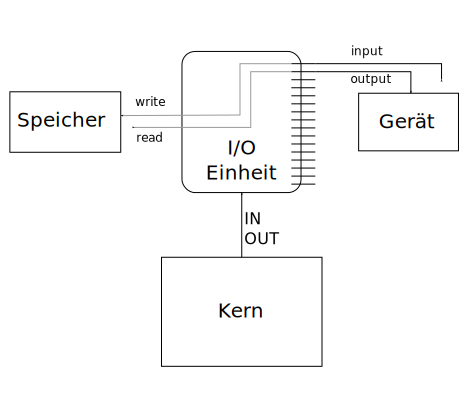
\includegraphics{./img/UMach-IO-Prozess.pdf}
 \caption{I/O wird von der I/O Einheit erledigt}
 \label{fig:UMach-IO-Prozess}
\end{figure}

Alle I/O Operationen finden zwischen dem Speicher und den Peripherie-Geräten
statt. Dabei wird der gesamte Datentransfer von der I/O-Einheit vermittelt und
gesteuert (siehe Abbildung \ref{fig:UMach-IO-Prozess} auf Seite
\pageref{fig:UMach-IO-Prozess}). Die I/O-Einheit besitzt zu diesem Zweck einen
direkten Zugriff auf den Speicher und kann dort unabhängig vom Kern lesen und
schreiben (Direct Memory Access, DMA\index{DMA}). Es ist zu bemerken, dass
der direkte Speicherzugriff von der I/O-Einheit unternommen wird und nicht von
den peripherischen Geräten selbst.

Alle I/O Operationen werden vom Kern unter Programmkontrolle angestoßen (siehe
auch Abschnitt \ref{sec:IO-Instruktionen} auf Seite
\pageref{sec:IO-Instruktionen}). Es werden also keine I/O Operationen
ausgeführt, die nicht explizit durch Maschinenbefehle angefordert werden.
Insbesondere werden keine I/O-Operationen aufgrund von
Unterbrechungsanfoderungen (interrupts) initialisiert.

Wenn ein I/O-Befehl ausgeführt wird, delegiert der Kern die Ausführung an die
I/O-Einheit und wartet, bis diese fertig ist. Erst wenn die I/O-Einheit
mit dem Transfer zwischen Speicher und Peripherie fertig ist, fährt der Kern mit
dem Programmablauf fort. Es werden parallel keine Instruktionen aus dem
Speicher geholt oder ausgeführt.


Die I/O-Einheit der UMach Maschine besteht aus einer Reihe von jeweils 8
Eingangs- und Ausgangschnittstellen, auch Ports\index{Port}\index{UMach!Port}
genannt. An diesen Ports können verschiedene physikalische Geräte angeschlossen
werden, welche die entsprechenden Daten generieren bzw. verarbeiten können.
(Siehe Abbildung \ref{fig:umach-aufbau} auf Seite \pageref{fig:umach-aufbau}.)


Die I/O Ports sind in zwei Kategorien unterteilt: 8 Eingabeports und 8
Ausgabeports. Von der Bauart und Struktur her, gibt es innerhalb der jeweiligen
Kategorie keine Unterschiede zwischen Ports. Sie werden lediglich anhand deren
Nummern identifiziert. Die Nummerierung der Ports fängt bei 0 an und wird bis
einschließlich Port 7 fortgeführt. 


Die Eingabe- und Ausgabefunktionen der I/O-Einheit werden durch
I/O-Instruktionen angefordert. Diese Instruktionen werden im Abschnitt
\ref{sec:IO-Instruktionen}, ab der Seite \pageref{sec:IO-Instruktionen}
beschrieben.


\paragraph{Bemerkung}
Zu diesem Entwicklungspunkt sind für die peripherischen Geräte, bzw. für die
entsprechenden Ports keine Kontrolle- oder Statusregister vorgesehen. Es gibt
auch keine entsprechende Befehle für die Kontrolle und Statusabfrage der
peripherischen Geräte. Es wird lediglich in den Speicher eingelesen und aus dem
Speicher ausgegeben. Eine zukünftige Version dieser Maschine könnte die
Kontrolle der peripherischen Geräte hinzufügen (wie z.B. ein- und ausschalten
der Geräte).




\begin{table}%no, this is not normal human being LaTeX
\newcolumntype{C}[1]{>{\ttfamily\footnotesize\centering\let\newline\\\arraybackslash\hspace{0pt}}p{#1}}
\newcolumntype{L}{>{\ttfamily\footnotesize}l}
\newcommand{\nhex}[1]{\multirow{2}{*}{#1}}
\centering
\caption[Befehlentabelle]
        {Befehlentabelle}
\label{tab:Befehlentabelle}
\begin{tabular}{|L||*{8}{C{1.2cm}|}}
\toprule\hline
          &   0   &   1   &   2   &   3    &   4    &   5    &    6    &    7    \\\hline\hline
\nhex{0}  &  NOP  &  RST  &  CRM  &  CSM   &  DIE   &  RSR   &  AUTSM  &  SOCL   \\\cline{2-9}
          & HATE  & TRST  &  ZMB  &  ALIV  &        &        &         &         \\\hline\hline
\nhex{1}  & SET   & SETU  & COPY  &  MOVE  &        &        &         &         \\\cline{2-9}
          &       &       &       &        &        &        &         &         \\\cline{1-9}
\nhex{2}  &  LB   &  LBU  &  LH   &  LHU   &  LW    &  LWU   &         &         \\\cline{2-9}
          &       &       &       &        &        &        &         &         \\\cline{1-9}
\nhex{3}  &  SB   &  SBU  &  SH   &  SHU   &  SW    &  SWU   &         &         \\\cline{2-9}
          &       &       &       &        &        &        &         &         \\\cline{1-9}
\nhex{4}  & PUSHB & PUSHH & PUSH  &        &        &        &         &         \\\cline{2-9}
          & POPB  & POPH  &  POP  &        &        &        &         &         \\\hline\hline
\nhex{5}  &  ADD  & ADDU  & ADDI  & ADDIU  &        &        &         &         \\\cline{2-9}
          &  SUB  & SUBU  & SUBI  & SUBIU  &        &        &         &         \\\cline{1-9}
\nhex{6}  &  MUL  & MULU  & MULI  & MULIU  &        &        &         &         \\\cline{2-9}
          &  DIV  & DIVU  & DIVI  & DIVIU  &        &        &         &         \\\cline{1-9}
\nhex{7}  &  MOD  &       & MODI  &        &        &        &         &         \\\cline{2-9}
          &  NEG  &  ABS  &  INC  &  DEC   &        &        &         &         \\\cline{1-9}
\nhex{8}  &       &       &       &        &        &        &         &         \\\cline{2-9}
          &       &       &       &        &        &        &         &         \\\hline\hline
\nhex{9}  &  AND  & ANDI  &  OR   &  ORI   &  XOR   &  XORI  &         &         \\\cline{2-9}
          & NAND  & NANDI &  NOR  &  NORI  &        &        &         &         \\\cline{1-9}
\nhex{A}  &  SHL  & SHLI  &  SHR  &  SHRI  &  SHRA  & SHRAI  &  ROTL   & ROTR    \\\cline{2-9}
          &  NOT  &       &       &        &        &        &         &         \\\hline\hline
\nhex{B}  &  CMP  & CMPU  & CMPI  & CMPIU  &        &        &         &         \\\cline{2-9}
          &       &       &       &        &        &        &         &         \\\hline\hline
\nhex{C}  &  BZ   &  BNZ  &  BLZ  &  BLEZ  &  BGZ   &  BGEZ  &         &         \\\cline{2-9}
          &  BEI  &  BNI  &  BLI  &  BLEI  &  BGI   &  BGEI  &         &         \\\cline{1-9}
\nhex{D}  &       &       &       &        &        &        &         &         \\\cline{2-9}
          &  JMP  &       &       &        &        &        &         &         \\\hline\hline
\nhex{E}  &  CALL &  RET  &       &        &        &        &         &         \\\cline{2-9}
          &       &       &       &        &        &        &         &         \\\hline\hline
\nhex{F}  &  WAKE &       &       &        &        &        &         &         \\\cline{2-9}
          &  KILL &       &       &        &        &        &         &         \\\hline\hline
          &   8   &   9   &   A   &   B    &   C    &   D    &    E    &    F    \\\hline
\bottomrule
\end{tabular}
\end{table} 



\appendix

\listoftables
\printglossary[title=Glossar,toctitle=Glossar,style=altlisthypergroup]
\printindex

\end{document}
